\subsection{Experimental setup along the evaluation path}
\label{sec:experiment-setup}

The experiments form a progression of questions, rather than one benchmark with a single configuration. The initial comparisons ask what the generated comment looks like beside a baseline. The prompt screen then separates writing instructions from the requirement to express a selected topic. Complete-message experiments test whether every carrier needed by the payload can be read, first with prepared context and then with independently acquired archive inputs. This is the logical organization of the evidence, not a claim that the samples form successive stages of one trial.

Figure~\ref{fig:evaluation-roadmap} maps these questions and the supporting checks.

\begin{figure}[H]
\centering
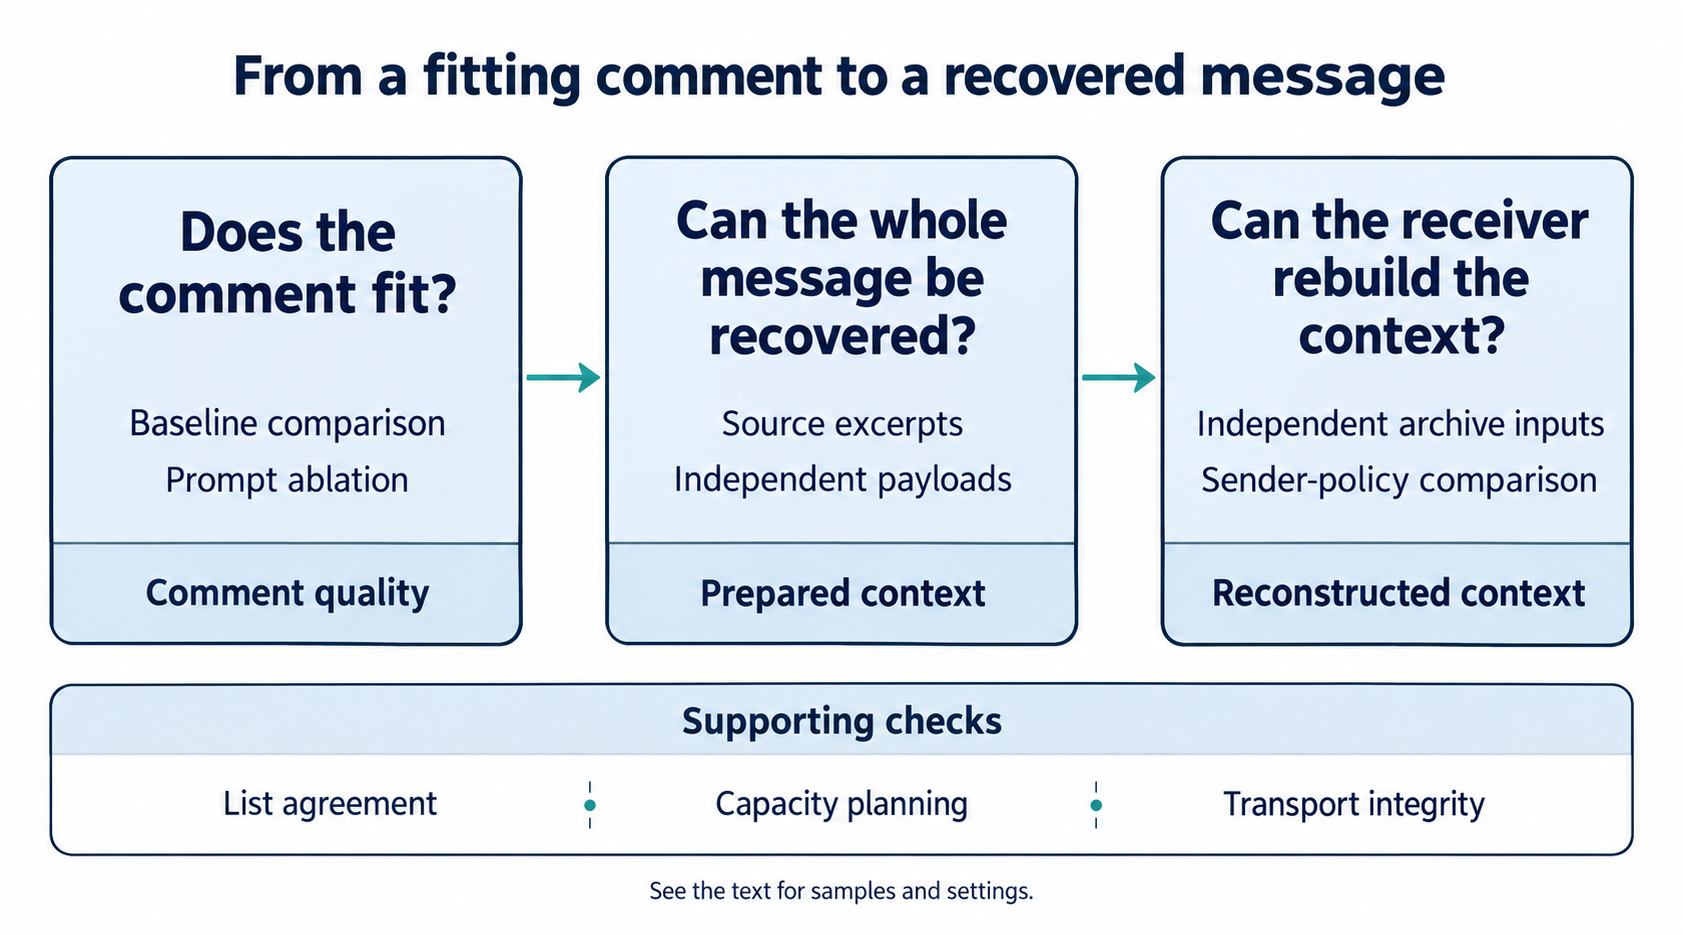
\includegraphics[width=\linewidth]{figures/evaluation_roadmap_en.png}
\caption{Evaluation organized by the question each experiment answers. Comment quality, complete-message recovery, and independent context reconstruction require different evidence. Supporting checks help locate failures; samples and configurations remain experiment-specific.}
\label{fig:evaluation-roadmap}
\end{figure}

Table~\ref{tab:experiment-setup} brings together the settings needed to interpret those changes. It complements the source-selection table and the outcome overview: those tables identify the populations and measurements, while this one identifies the model roles, generation budget, and receiving condition. An attempt means an initial generation call or a later retry; two attempts therefore mean one retry. The rationale for these settings is given beside the corresponding operations in Section~\ref{sec:model-settings}.

\begin{table}[H]
\centering\small
\caption{Configurations of the main live comparisons and recovery studies. Settings belong to the named experiment, not to every implementation of the method. A recorded model family is not a complete runtime identity.}
\label{tab:experiment-setup}
\renewcommand{\arraystretch}{1.12}
\begin{tabularx}{\linewidth}{|p{0.19\linewidth}|X|X|X|}
\hline
Experiment & Models and roles & Writing or attempt policy & Payload and receiving condition \\ \hline
Initial configuration comparison & Historical model/runtime identity is not fully pinned by the original result table. & Initial \texttt{context\_weighted\_v2} selection; 32-topic cap. & Single-comment selection; per-sample budget-based ZLG excerpts; assisted reconstruction. \\ \hline
Comment-quality comparison & Qwen 3.5 9B family for both generators; GPT-5.6 Luna, high reasoning, for judging. & Natural writing prompt; writer temperature 0.7; up to two generation attempts in the source campaign. & Single-comment comparison with audit-assisted reconstruction; five blinded judge criteria reuse 244 pairs. \\ \hline
Prompt-development screen & Generator identity not fully pinned by the screen manifests; GPT-5.6 Luna, high reasoning, for standout judgments. & G0--G5 and an argumentative variant; same 48 contexts and reply targets. & Topic-bearing candidates versus no-target writing controls; sender topic verification, not complete messages. \\ \hline
Source-excerpt recovery & Local Qwen 3.5 9B for generation and topic identification. & Anchored prompt; writer temperature 0.7; up to seven attempts per carrier and 12 carriers. & Dictionary-selected source excerpts; prepared lists and supplied carrier order. \\ \hline
Independent-payload development & GPT-6 Luna, low reasoning, through CLI; MiniLM retrieval. & Up to two attempts per carrier and 20 carriers; CLI temperature control unavailable. & Independent eight-byte messages; prepared context; receiver identifies topics through ordinary retrieval. \\ \hline
Archive reconstruction & Local Qwen 3.5 9B; GPT-OSS 20B for the later writing-quality check. & Anchored versus G5 at two attempts; later policies compare two and seven. Writer temperature 0.7, identifier 0, up to 20 carriers in the policy panels. & Independent eight-byte messages; thread-only extractive lists; each party fetches archive inputs independently. \\ \hline
\end{tabularx}
\end{table}

The local and CLI paths serve different experimental roles. The source-excerpt manifest records an NVIDIA GeForce RTX 5060 Ti with approximately 16 GB of device memory. The archive policy manifests identify the Qwen model served through LM Studio as Q4\_K\_M, with a loaded context of 16,384 tokens; that identity is specific to those panels. The official ZLG service uses its own token-probability runtime. Sharing the Qwen family in the quality comparison does not establish identical execution or computational budgets. Conversely, the CLI experiment requests a model and reasoning level without exposing an effective temperature setting, so current local defaults cannot be assigned to it retrospectively.

The writing conditions also need an explicit identity. The initial quality campaign uses the natural prompt package; source-excerpt recovery and the archive baseline use the anchored package, which directs the reply toward the selected topic in its parent context. G5 adds local conversational instructions and three fixed human-style examples, as detailed in Section~\ref{sec:prompt-ablation}. Topic construction and identification follow Sections~\ref{sec:methodology} and~\ref{sec:receiver-operation}; the exact quality-judge prompts appear in Appendix~\ref{app:judge-material}. The archive concision judge instead uses GPT-OSS 20B at temperature zero and presents both candidate orders, as described in Section~\ref{sec:fresh-archive}. These judging settings do not describe the carrier writer.

Preparation checks, the eight-carrier pilot, the reply-chain probe, and offline transport diagnostics support particular parts of this path. They retain their own inputs and budgets in Table~\ref{tab:evidence-levels} and their respective descriptions, rather than inheriting the configuration of a neighboring recovery study. Cost is likewise attached to an operation: acquiring and preparing sources, generating and checking candidates, selecting among accepted replies, or receiving carriers. Reusing prepared inputs excludes their acquisition cost from that measurement; summed model-call durations are not automatically end-to-end wall-clock latency.
